%!TEX root = ../template.tex
%!TEX root = ../template.tex
%%%%%%%%%%%%%%%%%%%%%%%%%%%%%%%%%%%%%%%%%%%%%%%%%%%%%%%%%%%%%%%%%%%%
%% Desenvolvimento.tex
%% NOVA thesis document file
%%
%% Chapter with content
%%%%%%%%%%%%%%%%%%%%%%%%%%%%%%%%%%%%%%%%%%%%%%%%%%%%%%%%%%%%%%%%%%%%

\typeout{NT FILE Desenvolvimento.tex}%

\prependtographicspath{{Chapters/Figures/}}

% epigraph configuration
\epigraphfontsize{\small\itshape}
\setlength\epigraphwidth{12.5cm}
\setlength\epigraphrule{0pt}

\chapter{Mapeamento dos Exames}
\label{cha:mapeamento_dos_exames}

%Este capítulo irá descrever como se procedeu ao mapeamento dos exames mais frequentes, que considerações foram tidas, que simplificações apresentam e o resultado final desta fase.\\

O processo de mapeamento dos exames começou com a decisão de quais incluir no estudo. Nem todos os exames foram considerados devido à baixa frequência com que estes ocorrem e a consequente falta de dados em relação à duração das suas atividades. Desta forma, apenas foram mapeados aqueles que ocorrem pelos menos mensalmente.\\
De seguida, foi necessário definir os recursos-tipo existentes no sistema, estes podem ser divididos em recursos humanos, técnicos auxiliares de saúde (TAS), enfermeiros, técnicos superiores de diagnóstico e terapêutica de medicina nuclear (TSDT), médicos especialistas (ME), e médicos cardiologistas (MC); e divididos em recursos físicos, gabinetes médicos (GB), sala de espera (SE), sala de espera de crianças (SEC), sala cortinas (SC), sala polivalente (SP), sala enfermagem 1 (SE1), sala enfermagem 2 (SE2), sala enfermagem 3 (SE3), sala câmara gama (SCG), e sala tomografo (ST).\\

\begin{table}[H]
\caption{Capacidade dos recursos humanos}
\label{tab:cap_RH}
\begin{tabular}{llllll}
\hline
Recurso-tipo & TAS & Enfermeiros & TSDT & ME & MC \\ \hline
Capacidade   & 4   & 4           & 4    & 2                     & 1
\end{tabular}
\end{table}

\begin{table}[H]
\caption{Capacidade dos recursos físicos}
\label{tab:cap_RFis}
\begin{tabular}{lllllllllll}
\hline
Recurso-tipo & GM & SE & SEC & SC & SP & SE1 & SE2 & SE3 & SCG & ST\\ \hline
Capacidade   & 2  & 4  & 3   & 2  & 1  & 1   & 3   & 3   & 1   & 1
\end{tabular}
\end{table}

Cada recurso-tipo tem uma quantidade de recursos disponíveis, para os recursos humanos corresponde ao número de profissionais em cada grupo existentes no departamento, para os recursos físico corresponde à lotação de pacientes que podem suportar, iremos considerar que existe portanto uma capacidade máxima para cada recurso-tipo, estas capacidades estão apresentadas na Tabela ~\ref{tab:cap_RH} e Tabela ~\ref{tab:cap_RFis}, respetivamente. Admite-se que cada recurso atribuído a uma tarefa será utilizado durante a duração total da atividade.\\
Considerou-se ainda a possibilidade de ter a capacidade dos recursos variável com o tempo, de forma a modelar os diferentes turnos e os períodos onde existe mudança entre estes. Contudo, com mais discussão decidiu-se que na prática dificilmente seria possível cumprir com uma agenda criada desta forma.\\

\begin{table}[H]
\caption{Capacidade dos recursos fictícios}
\label{tab:cap_RFic}
\begin{tabular}{lllllllllll}
\hline
Recursos fictícios & SP & SE1 & SP ou SE1 & SE2 & SE2 ou SE3\\ \hline
Capacidade         & 1  & 1   & 2         & 1   & 6
\end{tabular}
\end{table}

Existem recursos-tipo que podem ser equiparados a outros em certas atividades. A sala polivalente e sala enfermagem 1 podem ser tidas como equivalentes em certas atividades. Por isso foi necessário criar recursos-tipo fictícios. Para o exemplo anterior, foi criado o recurso-tipo sala polivalente ou sala enfermagem 1, sempre que uma destas salas é explicitamente necessária, a sua utilização é representadas no recurso-tipo correspondente e no recurso-tipo fictício, caso seja indiferente a sala necessárias, a utilização apenas é representada no recurso-tipo fictício. Contrariamente, a sala enfermagem 2 e sala enfermagem 3 podem também ser tidas como equiparadas, mas quando a sala enfermagem 2 é explicitamente necessária a sua capacidade é menor, passando de 3 para 1 pessoa, por isso o recurso fictício terá uma utilização de 3 lugares quando a sala de enfermagem 2 é necessária. Ambos os casos aparecem na Tabela ~\ref{tab:cap_RFic}, onde se observa a capacidade que será utilizada na sala de enfermagem 2.\\

Num passo seguinte, cada exame foi decomposto nas suas atividades. Considerou-se que uma nova atividade deve começar quando existe uma mudança dos recursos necessários. Foram então realizadas entrevistas de forma a realizar a decomposição dos exames, no seguimento das entrevistas as atividades foram validadas pelos vários grupos profissionais. Rapidamente identificou-se a necessidade de diferenciar o mapeamento entre pacientes com mobilidade autónoma, e aqueles com mobilidade condicionada, e crianças, existindo diferenças nos recursos necessários e na duração de cada atividade.\\
Seguidamente, as duração de cada atividade foram recolhidas utilizando folhas de registo provenientes do mapeamento realizado. A duração média de cada atividade foi obtida através da hora de início e de fim de cada atividade registadas pelos profissionais, será de salientar que mesmo sendo este um problema de \textit{No-Wait}, nem sempre foi verificado nas folhas de registo, evidenciando um possível relaxamento da restrição.\\
Todas as folhas de registo e respetivos dados estarão em anexo com esta dissertação.\\

\chapter{Desenvolvimento dos Modelos}
\label{cha:desenvolvimentos_dos_modelos}

Este capítulo os três problemas que devem ser resolvidos, para tal foram desenvolvidos vários modelos. No primeiro problema existem recursos e exames fixos, sendo o objetivo minimizar o tempo entre o começo e o fim de todos os exames, chamado de \textit{makespan}. O segundo problema tem recursos e tempo fixos, sendo o objetivo maximizar o número de exames a realizar, utilizando um somatório simples ou ponderado. Finalmente, o terceiro problema é caracterizado por exame e tempos fixos, sendo o objetivo minimizar os recursos necessários para realizar todos os exames no tempo definido.

\section{Problema de \textit{Makespan}}

Este problema irá utilizar o exemplo de uma segunda-feira típica em termos de exames realizados. Ocorrendo três cintigrafia tiroideia, cinco cintigrafia pulmonar de ventilação/inalação + perfusão, dez cintigrafia miocárdica de perfusão em repouso, uma cintigrafia das glândulas salivares, e dez PET-FDG.\\
A próxima formulação é a que tradicionalmente se encontra quando indexada no tempo, chamá-la-emos de \textit{MILP-trad}:\\

Conjuntos:\\
O conjunto de trabalhos $I, i \in I := (1, \ldots, n)$ \\
O conjunto de operações $K, k \in K := (1, \ldots, K_{\max})$ \\
O conjunto de recursos-tipo $R, p \in R := (1, \ldots, R_{\max})$ \\
O conjunto de instantes de tempo $T, t \in T := (1, \ldots, T_{\max})$ \\

Parâmetros:\\
$\rho_{i,k}$ é o tempo de processamento da operação $k$ do trabalho $i$ \\
$r_{i,p,k}$ é o número de recursos $p$ necessários para realizar a operação $k$ do trabalho $i$ \\
$C_{p}$ é a capacidade do recursos do tipo $p$ \\

Variáveis de Decisão: \\
$X_{t,i,k}$ é uma variável binária com valor 1 se a operação $k$ do trabalho $i$ ocorrer durante o instante $t$, caso contrário tem valor 0 \\
$Z_{t,i,k}$ é uma variável binária com valor 1 se a operação $k$ do trabalho $i$ começar no instante $t$, caso contrário tem valor 0 \\
$S_{i,k}$ é uma variável inteira que representa o valor de começo da operação $k$ do trabalho $i$ \\
$F_{i,k}$ é uma variável inteira que representa o valor de fim da operação $k$ do trabalho $i$ \\
$C_{\max}$ é uma variável inteira que representa o \textit{makespan} \\

Função Objetivo:
\begin{align}
\min C_{\max} \label{eq:1}
\end{align}

Sujeito a:
\begin{align}
&F_{i,K_{\max}} \leq C_{\max} \quad \forall i \label{eq:2} \\
&\sum_{t}Z_{t,i,k} = 1 \quad \forall i,k \label{eq:3} \\
&\sum_{t}X_{t,i,k} = \rho_{i,k} \quad \forall i,k \label{eq:4} \\
&\sum^{t+\rho_{i,k}}_{t^{'}=t}X_{t^{'},i,k} \geq \rho_{i,k}Z_{t,i,k} \quad \forall i,k,t=1, \ldots,T-\rho_{i,k} \label{eq:5} \\
&S_{i,k} = \sum_{t}tZ_{t,i,k} \quad \forall i,k \label{eq:6} \\
&S_{i,k+1} = F_{i,k} \quad \forall i,k \label{eq:7} \\
&F_{i,k} - S_{i,k} = \rho_{i,k} \quad \forall i,k \label{eq:8} \\
&\sum_{i}\sum_{k}r_{i,p,k}X_{t,i,k} \leq C_{p} \quad \forall t,p \label{eq:9} 
\end{align}
A função objetivo (~\ref{eq:1}) minimiza o \textit{makespan} dos trabalho, ou seja, o tempo entre o início do primeiro exame, e o fim do último.\\
A restrição (~\ref{eq:2}) garante que todos os trabalho acabam antes ou no instante do \textit{makespan}, auxiliando a função objetivo.\\
A restrição (~\ref{eq:3}) garante que só existe um instante em que a operação $k$ do trabalho $i$ é atribuído.\\
A restrição (~\ref{eq:4}) garante que para a operação $k$ do trabalho $i$ o somatório de $X_{t,i,k}$ sobre $t$ tem o valor da duração $\rho_{i,k}$. \\
A restrição (~\ref{eq:5}) garante a concordância do posicionamento sobre $t$ entre $X_{t,i,k}$ e $Z_{t,i,k}$. \\
A restrição (~\ref{eq:6}) garante a coerência do momento de início da tarefa $k$.\\
A restrição (~\ref{eq:7}) garante que para o trabalho $i$ a operação $k+1$ começa quando a operação $k$ acaba, verificando a restrição de \textit{No-Wait}. \\
A restrição (~\ref{eq:8}) garante que a duração da operação $k$ para o trabalho $i$ é de $\rho_{i,k}$.\\
A restrição (~\ref{eq:9}) garante que não existe a sobre-utilização do recursos $p$ durante o instante $t$m verificando as extensões \textit{Multi-Resource} e \textit{Flexible}.\\

Por outro lado, é possível formular modelos mais eficientes que este clássico. Isto poderá ser feito com o pré-processamento de cada trabalho, permitindo inserir cada trabalho na sua totalidade e verificar se este irá causar sobre-utilização de recursos, chamá-la-emos de \textit{MILP-$\delta$}.\\

Por outro lado, será possível formular modelos mais eficientes que o clássico. A formulação aqui sugerida, \textit{MILP-$\delta$}, tira partido do facto da restrição \textit{No-Wait} criar um padrão de utilização de recursos, qualquer que seja o instante $t$ onde este se insere. Desta forma não é necessário explicitamente formular restrições que garantem \textit{No-Wait}.\\

Conjuntos:\\
O conjunto de trabalhos $I, i \in I := (1, \ldots, n)$ \\
O conjunto de recursos-tipo $R, p \in R := (1, \ldots, R_{\max})$ \\
O conjunto de instantes de tempo $T, t \in T := (1, \ldots, T_{\max})$ \\

Parâmetros:\\
$\rho_{i}$ é duração do trabalho $i$ \\
$\delta_{i}(u,p)$ é a quantidade de recursos do tipo $p$ necessários a um offset de $u$ instantes de tempo no trabalho $i$\\
$C_{p}$ é a capacidade do recursos do tipo $p$ \\

Variáveis de Decisão: \\
$Z_{t,i}$ é uma variável binária com valor 1 se o trabalho $i$ começar no instante $t$, caso contrário tem valor 0 \\
$F_{i}$ é uma variável inteira que representa o valor de fim do trabalho $i$ \\
$C_{\max}$ é uma variável inteira que representa o \textit{makespan} \\

Função Objetivo:
\begin{align}
\min C_{\max} \label{eq:10}
\end{align}

Sujeito a:
\begin{align}
&F_{i} \leq T_{\max} \quad \forall i \label{eq:11} \\
&\sum^{T_{\max}-\rho_{i}+1}_{t=0}Z_{t,i} = 1 \quad \forall i \label{eq:12} \\
&\sum^{T_{\max}-\rho_{i}+1}_{t=0}Z_{t,i}*(t+\rho_{i}) = F_{i} \quad \forall i \label{eq:13} \\
&\sum_{i}\sum^{\min(t, T_{\max}-\rho_{i})}_{\tau=\max(0, t-\rho_{i}+1)}\delta_{i}(t-\tau,p)Z_{\tau,i} \leq C_{p} \quad \forall t,p \label{eq:14}
\end{align}
A função objetivo (~\ref{eq:10}) minimiza o \textit{makespan} dos trabalho.\\
A restrição (~\ref{eq:11}) garante que todos os exames acabam antes ou no instante do \textit{makespan}, auxiliando a função objetivo.\\
A restrição (~\ref{eq:12}) garante que só existe um instante de começo do trabalho $i$.\\
A restrição (~\ref{eq:13}) faz a ligação entre as variáveis $Z_{t,i}$ e $F_{i}$.\\
A restrição (~\ref{eq:14}) garante que não há sobre utilização de recursos, ao verificar para cada instante $t$ quais trabalhos estão a ser executados e em que fase este se encontra, garantindo que em cada instante não há sobre-utilização de recursos.\\

Para ambas das formulações apresentadas, o tamanho do conjunto de instantes de tempo, $T$, tem impacto no número de variáveis e restrições, será por isso importante encontrar o menor valor de $T_{\max}$ possível mas que seja maior que \textit{makespan}, a isto tipicamente chama-se de \textit{upper-bound}. No decorrer desta secção demonstrar-se-à o impacto que este valor tem nas formulações apresentadas.\\ 

De seguida foram desenvolvidos três modelos com duas codificações de solução diferentes. Os dois primeiros modelos utilizam uma codificação que representa o instante de início de cada trabalho. O outro modelo utiliza a sequencia de escalonamento de cada trabalho como solução.\\

\subsection{Modelo 1}

Este modelo é definido pelo o facto de não existir a garantia da viabilidade de cada solução. Por isso à partida será necessário criar uma função objetivo diferente das restante, esta será dada por:
$$f(s) = C_{\max} + P \sum_{t=start}^{end-1}\sum_{p}v(t,p)$$
Onde $C_{\max}$ é \textit{makespan}, $P$ a punição relativamente à sobre-utilização de recursos (sendo esta uma variável a estudar), esta sobre-utilização é dada pelo somatório sobre os recursos e instantes de tempo, $v(t,p)$ por sua vez é dado por:
$$
v(t,p)=
\begin{cases}
	1 & \text{se } u(t,p)>C_{p}\\
	0 & \text{caso contrário}
\end{cases}
$$
Temos que $u(t,p)$ é a utilização de cada recurso $p$ em cada instante $t$, $C_{p}$ será a capacidade máxima de cada recurso. Poderia ter-se considerado uma definição diferente de $v(t,p)$, mas que apresentou resultados piores.\\
$$
v(t,p)=
\begin{cases}
	u(t,p)-C_{p} & \text{se } u(t,p)>C_{p}\\
	0            & \text{caso contrário}
\end{cases}
$$

Será de saliente como $C_{\max}$ é calculado, existem duas formas semelhantes para tal. A primeira considera que $C_{\max}$ é dado pelo valor máximo do término de cada trabalho. A segunda será pela diferença entre o valor máximo de término de cada trabalho e o valor mínimo de início de cada trabalho. Apesar de aparentemente iguais, a diferença deste cálculo terá impacto na procura e avaliação de cada vizinho.\\
\begin{figure}[H]
	\centering
	\begin{subfigure}{0.49\textwidth}
	\centering
		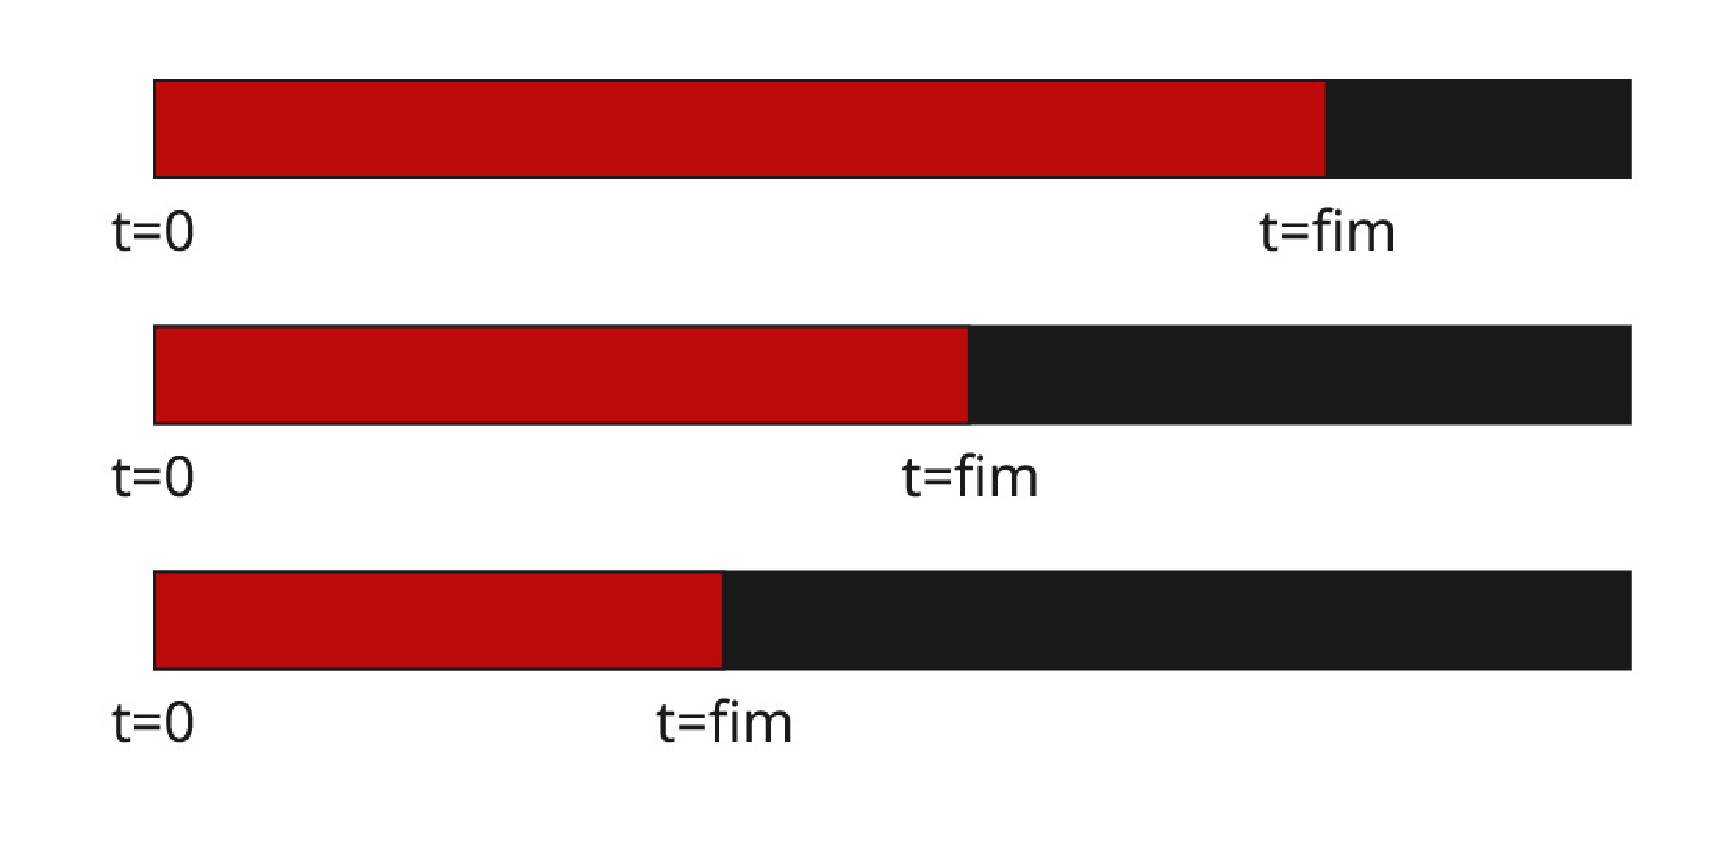
\includegraphics[width = \textwidth]{0_makespan}
		\caption{}
		\label{fig:dif_makespan_a}
	\end{subfigure}
	\begin{subfigure}{0.49\textwidth}
	\centering
		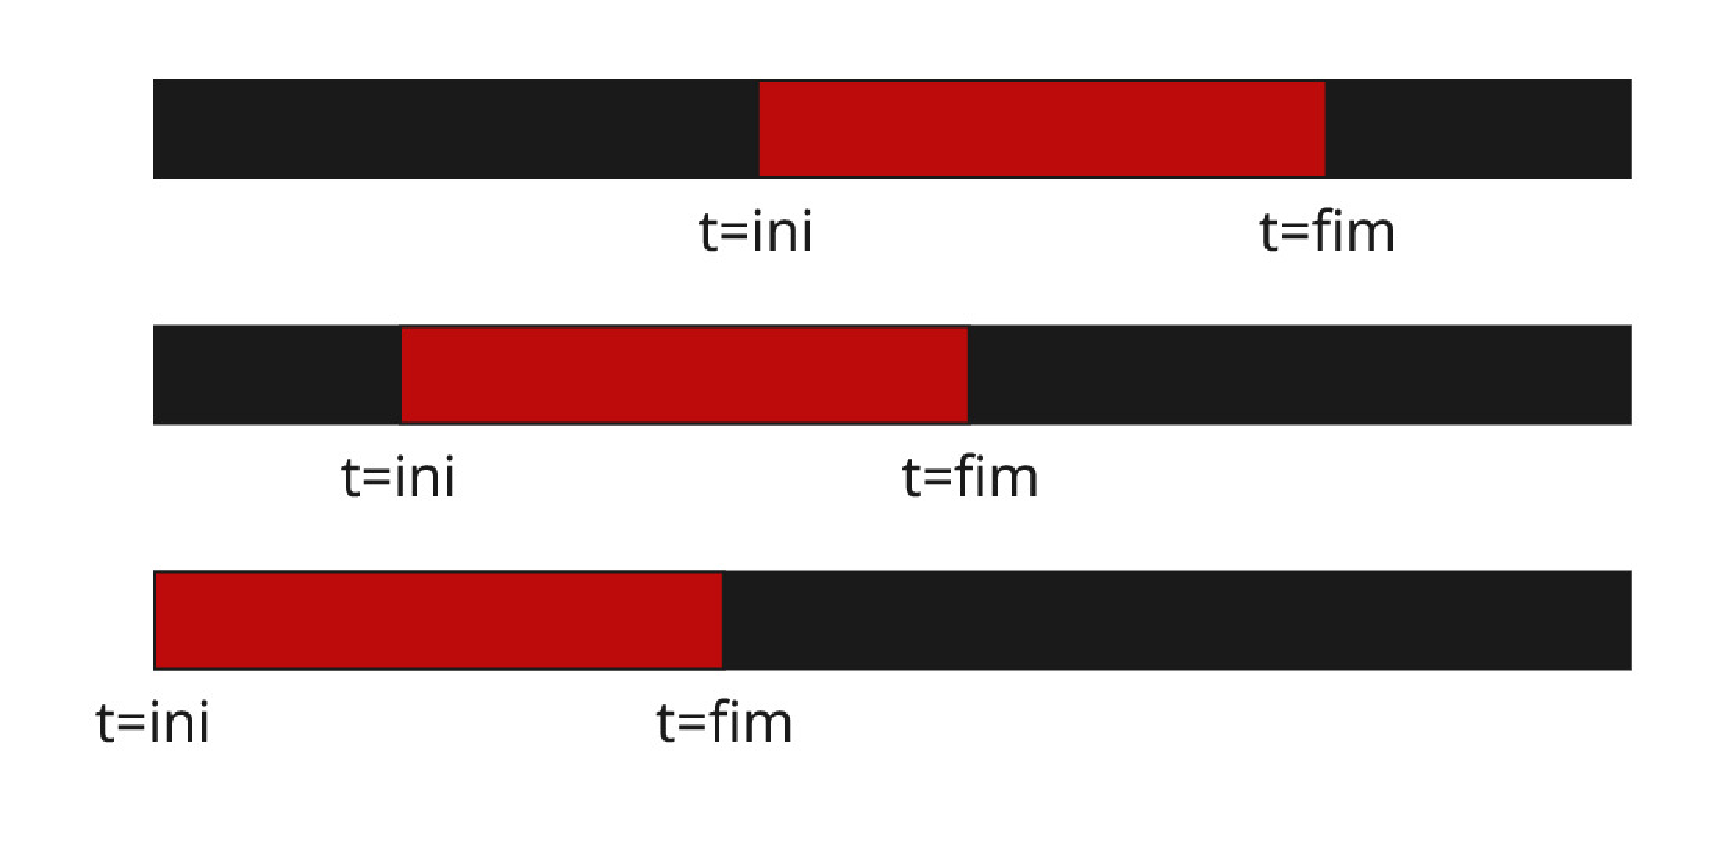
\includegraphics[width = \textwidth]{start_end}
		\caption{}
		\label{fig:dif_makespan_b}
	\end{subfigure}
	\caption{Impacto das diferentes formas de calcular $C_{\max}$}
	\label{fig:dif_makespan}
\end{figure}
A figura~\ref{fig:dif_makespan} apresenta três agendas diferentes, a vermelho temos o valor de \textit{makespan} de cada agenda, na figura~\ref{fig:dif_makespan_a} temos que \textit{makespan} é dado pelo máximo do término de cada trabalho, enquanto na figura~\ref{fig:dif_makespan_b} temos que \textit{makespan} é dado pela diferença entre o valor máximo de término de cada trabalho e o valor mínimo de início de cada trabalho. Nesta primeira figura as três agendas têm valores diferentes de $f(s)$, a segunda figura apresenta três agendas com o mesmo valor de $f(s)$.\\
\begin{figure}[H]
	\centering
	\begin{subfigure}{0.49\textwidth}
	\centering
		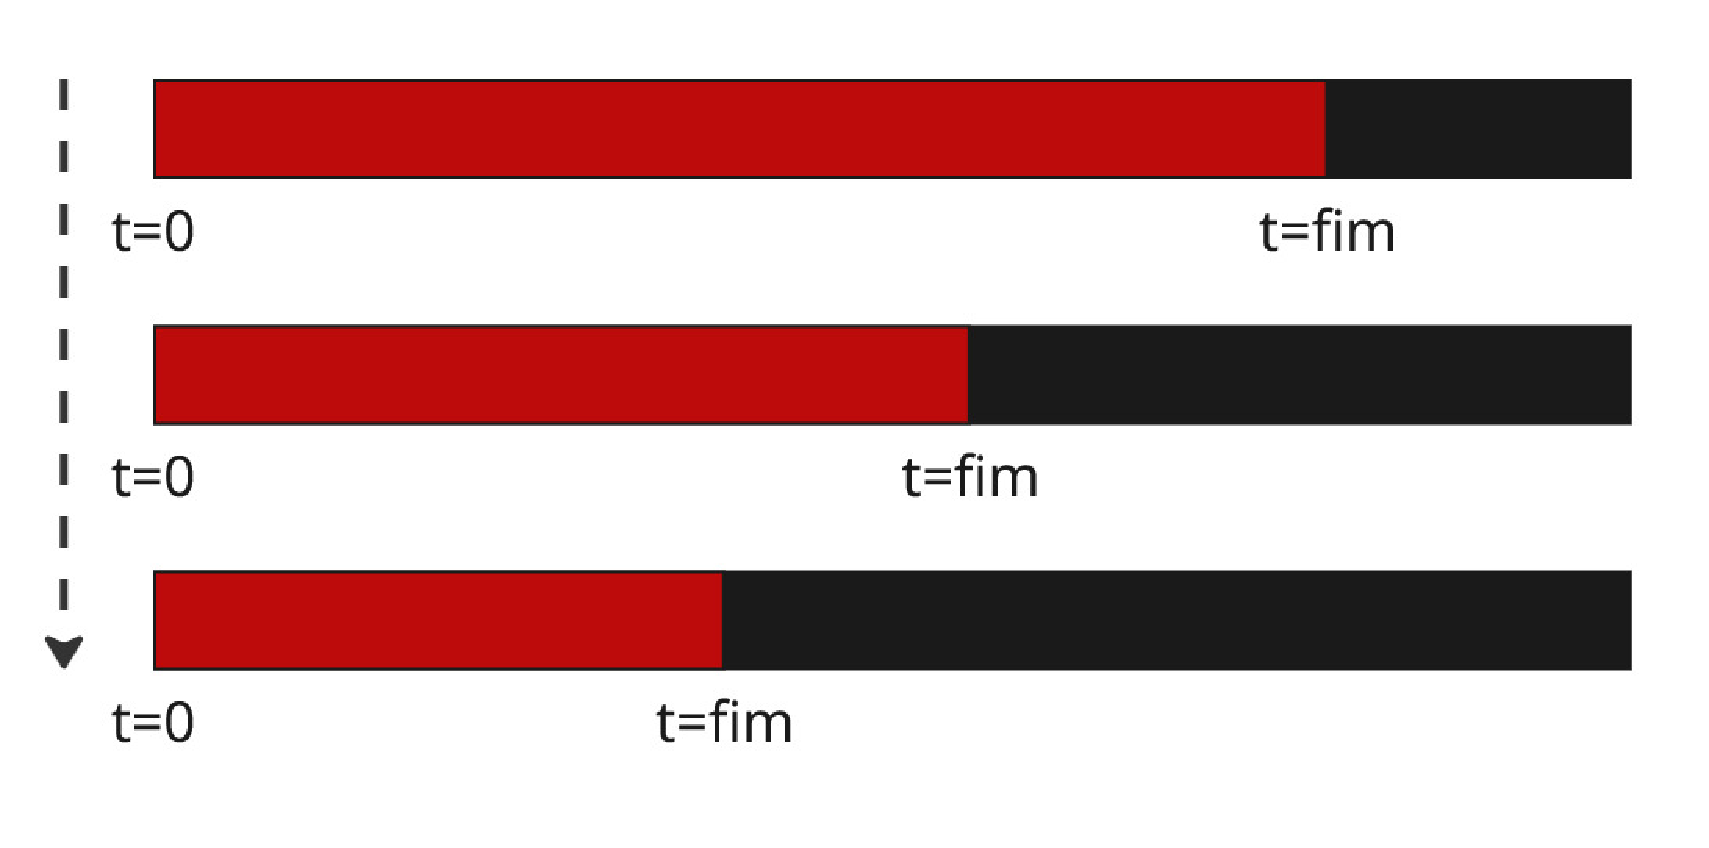
\includegraphics[width = \textwidth]{U(0_makespan)}
		\caption{}
		\label{fig:dif_uniform_a}
	\end{subfigure}
	\begin{subfigure}{0.49\textwidth}
	\centering
		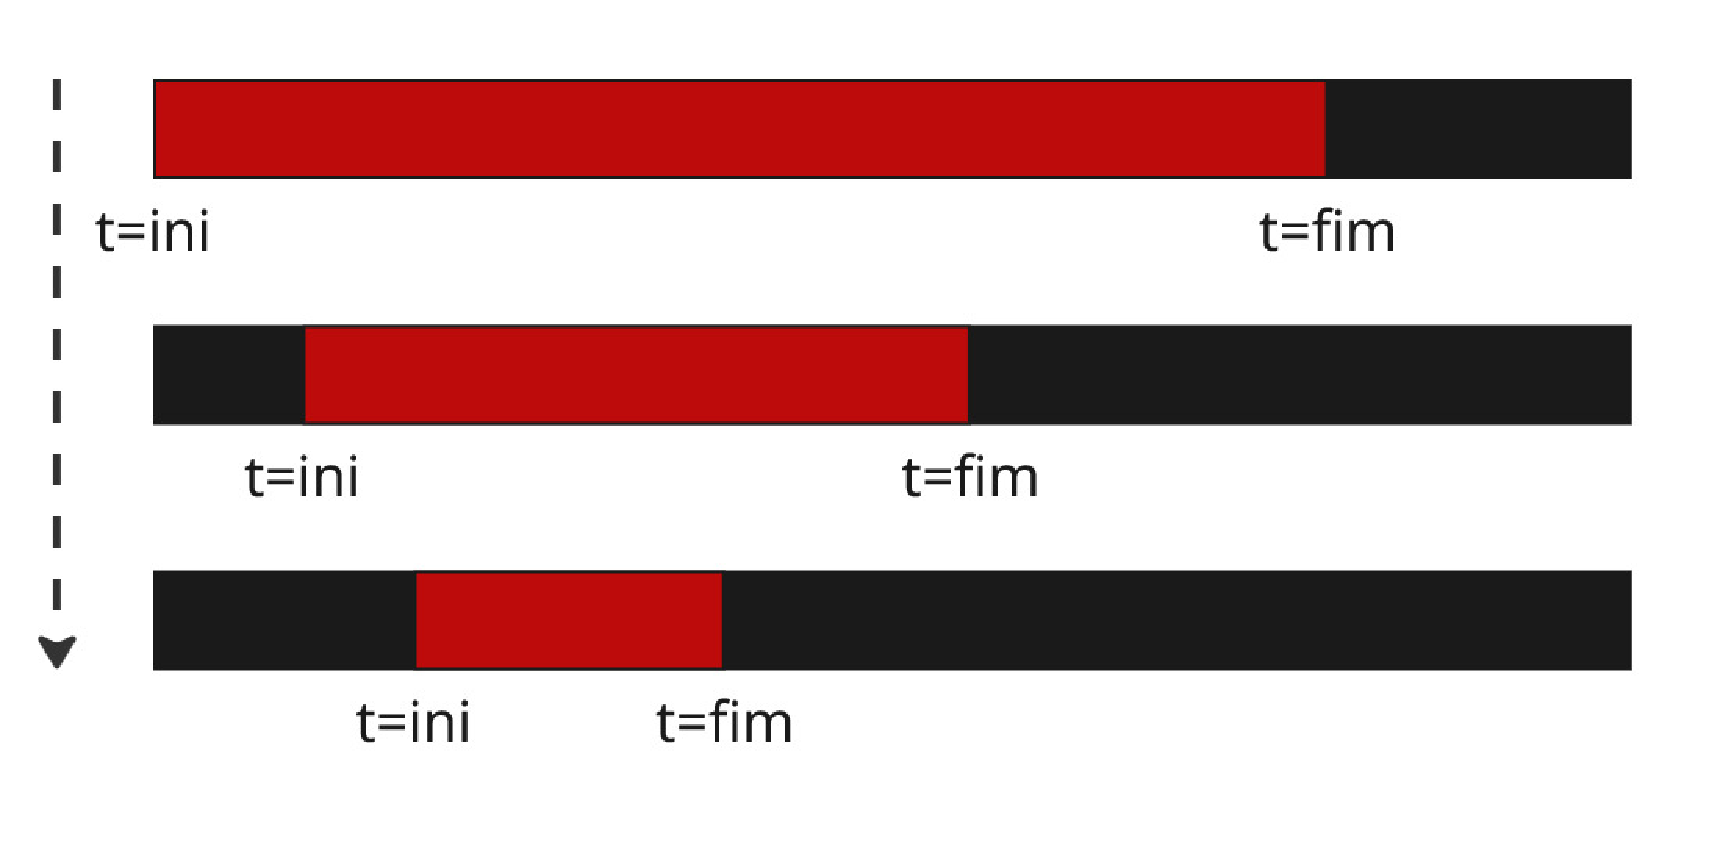
\includegraphics[width = \textwidth]{U(start_end)}
		\caption{}
		\label{fig:dif_uniform_b}
	\end{subfigure}
	\caption{Impacto na procura da vizinhança na geração de um novo instante $t$}
	\label{fig:dif_uniform}
\end{figure}
Para este modelo, a solução $s$ é dada pelo instante $t$ em que começa cada trabalho $i$. Por sua vez, a vizinhança de $s$, $\mathcal{N}(s)$, é definida pelo trabalho a reagendar e quando este deve começar, $(i, t)$. Ambos estes valores são obtidos aleatoriamente, contudo $t$ poderá ser obtido através de uma uniforme U(0, \textit{makespan}-duração), ou U(start, end-duração), sendo a duração o tempo a completar o trabalho $i$ selecionado. Esta diferença aparentemente pequena gera soluções finais bastante diferentes.\\
Podemos utiliza a figura~\ref{fig:dif_uniform} para perceber o porquê. Observamos uma sequencia no tempo da otimização de uma agenda, em que na figura~\ref{fig:dif_uniform_a} se utiliza U(0, \textit{makespan}-duração) na geração de novos vizinhos, e na figura~\ref{fig:dif_uniform_b} se utiliza U(start, end) na geração de novos vizinhos. Em ambas existe a diminuição de \textit{makespan} quando se agenda o último trabalho para um instante inferior. Contudo apenas utilizando U(start, end-duração) para gerar os instantes, se poderá tirar proveito de agendar o primeiro trabalho para um instante superior. Utilizar-se-à o mecanismo descrito como \textbf{NE1}~\cite{franzinRevisitingSimulatedAnnealing2019}.
\begin{figure}[H]
	\centering
	\makebox[\textwidth][c]{%
		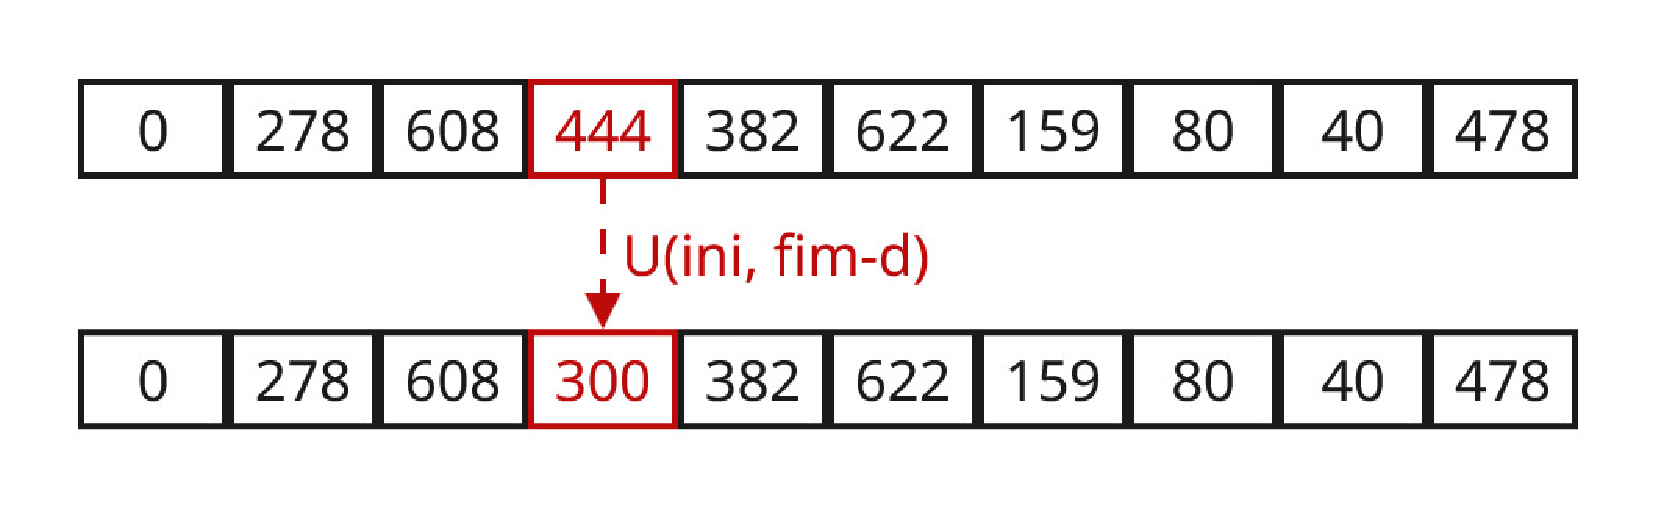
\includegraphics[width=0.5\textwidth]{P1M1_NGV_viz}
	}
	\caption{Processo de transição da solução $s$ para a solução $s'$}
	\label{fig:trans_P1M1_NGV}
\end{figure}
O processo de modificar a solução atual $s$ de forma a obter uma nova solução $s'$ da vizinhança é resumido à figura~\ref{fig:trans_P1M1_NGV}. Sendo depois necessário calcular $f(s')$. O pseudo-código abaixo descreve este processo.\\
\begin{algorithm}[H]
    $i \gets$ U(0,$n$)\;
    $q \gets U(0,1)$\;
    $\delta \gets$ tipo\_exame\_delta[i]\;
    \tcp{$\delta$ é uma matriz com os recursos ao longo da duração do trabalho $i$}
    $d \gets$ duração[i]\;
    ini\_velho $\gets S[i, 0]$\;
    ini\_novo $\gets$ U(ini, fim-d)\;
    \tcp{ini e fim provenientes da iteração anterior}
    salto $\gets$ ini\_novo-ini\_velho\;
    \For{$k \gets 0$ \KwTo n\_operações}
    {
    $S[i, k] \gets S[i, k]+ \text{salto}$\;
    $F[i, k] \gets F[i, k]+ \text{salto}$\;
    \tcp{$S$ e $F$ são matrizes com o instante $t$ de início e fim de cada trabalho $i$ e operação $k$}
    }
	\For{$t \gets 0$ \KwTo $d$}
	{
    	\For{$p \gets 0$ \KwTo n\_recursos}
    	{
		$u[t+\text{ini\_velho}, p] \gets u[t+\text{ini\_velho}, p] - \delta[t, p]$\;
		$u[t+\text{ini\_novo}, p] \gets u[t+\text{ini\_novo}, p] + \delta[t, p]$\;
    	}
	}
    ini $\gets \min(S)$\;
    fim $\gets \max(F)$\;
    $C_{\max} \gets \text{fim} - \text{ini}$\;
    $f(s') \gets C_{\max} + P \sum_{t=start}^{end-1}\sum_{p}v(t,p)$\;
    \If{$f(s')<f(s)$ ou $q < exp(-(f(s)-f(s'))/c)$}
	{
		$s \gets s'$
	}
	\Else
	{
	\For{$k \gets 0$ \KwTo n\_operações}
    {
    $S[i, k] \gets S[i, k]- \text{salto}$\;
    $F[i, k] \gets F[i, k]- \text{salto}$\;
    }
	\For{$t \gets 0$ \KwTo $d$}
	{
    	\For{$p \gets 1$ \KwTo n\_recursos}
    	{
		$u[t+\text{ini\_velho}, p] \gets u[t+\text{ini\_velho}, p] + \delta[t, p]$\;
		$u[t+\text{ini\_novo}, p] \gets u[t+\text{ini\_novo}, p] - \delta[t, p]$\;
    	}
	}
	}
    \caption{Pseudo-código de gerção de novos vizinhos, a sua avaliação, aceitação ou rejeição. Modelo 1.}
\end{algorithm}

A temperatura inicial segue o esquema \textbf{IT6}~\cite{franzinRevisitingSimulatedAnnealing2019}. Mais especificamente, gerou-se uma boa solução inicial utilizando a heurística NEH, e de seguida procedeu-se a uma caminhada aleatório da vizinhança desta solução utilizando $c=\infty$ e $L_k=100000$, de forma a aceitar todas as novas soluções encontradas. Definindo-se então que a temperatura inicial é dada por:
$$c_{0}=|\Delta_{avg}/log(p_{0})|$$
Onde $\Delta_{avg}$ é a diferença média entre a solução atual $s$ e o vizinho $s'$, e $p_{0}$ é a probabilidade inicial de aceitar cada solução, este último valor será uma das variáveis a estudar.\\
O critério de paragem utilizado foi uma modificação de \textbf{SC9}~\cite{franzinRevisitingSimulatedAnnealing2019}, onde se termina o algoritmo quando um número fixo de reduções de temperatura não geram novas soluções melhores, este valor será uma das variáveis a estudar.\\
O critério de aceitação utilizado foi o tradicional descrito por Metropolis~\cite{metropolisEquationStateCalculations1953}, ou seja, \textbf{AC1}~\cite{franzinRevisitingSimulatedAnnealing2019}.\\
O esquema de arrefecimento utilizado foi \textbf{CS2}~\cite{franzinRevisitingSimulatedAnnealing2019}, dado por $c_{k+1}=\alpha c_{k}$, $\alpha$ tipicamente é um valor perto de 1, de forma a que a redução da temperatura se dê lentamente, este valor será uma das variáveis a estudar.\\
O comprimento da temperatura, ou seja, $L_{k}$, será uma variável a estudar, adotou-se o critério \textbf{TL1}~\cite{franzinRevisitingSimulatedAnnealing2019}, considerando um número fixo de iterações durante cada redução de temperatura.\\

Existem três diferentes algoritmos considerados para a geração da solução inicial, um algoritmo \textit{greedy}, um algoritmo aleatório, e a heurística NEH. O primeiro agenda cada trabalho aleatoriamente de forma a que o fim do trabalho $i$ corresponde ao início do trabalho $i+1$, garantindo que esta solução não apresenta sobre-utilização de recursos. O segundo agenda cada trabalho de forma aleatória, sem atender à possível sobre-utilização de recursos. Verificou-se que o segundo algoritmo apresenta, na sua generalidade, melhores soluções em relação ao primeiro algoritmo.\\
\begin{figure}[h]
    \centering
    % Row 1
    \begin{subfigure}{0.49\textwidth}
        \centering
        \includegraphics[width=\textwidth]{P1M1_NGV_makespan_greedy}
        \caption{}
        \label{fig:P1M1_NGV_makespan_greedy}
    \end{subfigure}
    \hfill
    \begin{subfigure}{0.49\textwidth}
        \centering
        \includegraphics[width=\textwidth]{P1M1_NGV_makespan_greedy_clip}
        \caption{}
        \label{fig:P1M1_NGV_makespan_greedy_clip}
    \end{subfigure}
    
    % Row 2
    \begin{subfigure}{0.49\textwidth}
        \centering
        \includegraphics[width=\textwidth]{P1M1_NGV_makespan_random}
        \caption{}
        \label{fig:P1M1_NGV_makespan_random}
    \end{subfigure}
    \hfill
    \begin{subfigure}{0.49\textwidth}
        \centering
        \includegraphics[width=\textwidth]{P1M1_NGV_makespan_random_clip}
        \caption{}
        \label{fig:P1M1_NGV_makespan_random_clip}
    \end{subfigure}
    
    % Row 3
    \begin{subfigure}{0.49\textwidth}
        \centering
        \includegraphics[width=\textwidth]{P1M1_NGV_makespan_NEH}
        \caption{}
        \label{fig:P1M1_NGV_makespan_NEH}
    \end{subfigure}
    \hfill
    \begin{subfigure}{0.49\textwidth}
        \centering
        \includegraphics[width=\textwidth]{P1M1_NGV_makespan_NEH_clip}
        \caption{}
        \label{fig:P1M1_NGV_makespan_NEH_clip}
    \end{subfigure}
    \caption{Evolução do valor da função objetivo ao longo da otimização do problema \textit{makespan} com o modelo 1, para a obtenção destas figuras, as variáveis utilizadas foram: $L_{k}=5000$, $CP=100$, $\alpha=0.8$, $P=1000$, $p_{0}=0.9$.}
    \label{fig:P1M1_NGV_dif_sol_ini}
\end{figure}
Podemos observar a figura~\ref{fig:P1M1_NGV_dif_sol_ini} de acordo com o comportamento de cada solução e o porquê de rejeitarmos a heurística NEH como solução inicial. Em todos os algoritmos observa-se um pico da função objetivo, este facto deve-se à elevada temperatura inicial, levando consequente à aceitação da maioria das soluções candidatas, permitindo haver alguma independência entre a solução inicial e a final. Com o decair da temperatura a aceitação contrai, havendo aqui grande parte da melhoria observada. Quando a temperatura é muito reduzida, \textit{SA} transforma-se numa simples procura local, ao tornar-se quase impossível aceitar soluções piores que a atual.\\
Apesar da heurística NEH apresentar uma boa solução inicial, este facto torna-se prejudicial no decorrer do \textit{SA}, porque dificilmente haverá uma solução melhor que a inicial nas primeiras reduções de temperatura, podendo nunca melhorar até que o critério de paragem seja acionado.\\
As temperaturas iniciais encontradas são muito elevadas, $\Delta_{avg}$ é elevado devido à grande probabilidade que cada solução gerada ter vários instantes com sobre-utilização de recursos.

Será de realçar ainda duas peculiaridades deste modelo. Depois da redução da temperatura, o primeiro vizinho terá de ter o seu instante $t$ gerado utilizando U(0,$T_{\max}$-duração), sendo $T_{\max}$ o somatório das durações de todos os trabalhos,caso contrário o algoritmo parece não funcionar.\\
Na rejeição de uma solução deveria-se recalcular o início e o fim da agenda, de forma a que, na próxima iteração, o novo instante gerado corresponda corretamente à solução atual. Contudo isto resulta em piores soluções finais, isto será devido à pressão criada pela geração de um novo instante com menor \textit{makespan}.\\
\begin{figure}[H]
	\centering
	\begin{subfigure}{0.49\textwidth}
	\centering
		\includegraphics[width = \textwidth]{P1M1_NGV_walkback_orig}
		\caption{}
		\label{fig:P1M1_NGV_walkback_orig}
	\end{subfigure}
	\begin{subfigure}{0.49\textwidth}
	\centering
		\includegraphics[width = \textwidth]{P1M1_NGV_walkback_alt}
		\caption{}
		\label{fig:P1M1_NGV_walkback_alt}
	\end{subfigure}
	\caption{Impacto na procura da vizinhança na geração de um novo instante $t$}
	\label{fig:P1M1_NGV_walkback}
\end{figure}
Na figura~\ref{fig:P1M1_NGV_walkback}, a primeira agenda tem $\textit{makespan}=\text{fim}-\text{ini}$, e por isso o vizinho terá um novo instante gerado por U(ini, fim-duração), a segunda agenda mostra as fronteiras depois de se rejeitar a solução, a terceira agenda em~\ref{fig:P1M1_NGV_walkback_orig} irá gerar o novo instante numa secção mais restrita da agenda, guiando \textit{makespan} para ser menor, por sua vez em~\ref{fig:P1M1_NGV_walkback_alt} toda a amplitude de \textit{makespan} é considerada. Este é o único mecanismo de enviesamento da solução neste modelo.\\

\subsection{Modelo 2}

Este modelo é semelhante ao anterior, contudo já existe garantia da viabilidade de cada solução durante a geração da vizinhança. Desta forma, a função objetivo é mais simples, e é dada por:\\
$$f(s) = C_{\max}$$
Sendo $C_{\max}$ o valor de \textit{makespan} calculado como anteriormente, a diferença entre o máximo de término de cada trabalho e o valor mínimo de início de cada trabalho.\\

A codificação utilizada para este modelo é igual à do modelo anterior. Contudo a forma de gerar o novo instante $t$ em que o trabalho $i$ deve começar difere substancialmente.\\
Como existe garantia da viabilidade da solução, ou seja, todas a restrições são obedecidas, não podemos selecionar qualquer instante $t$ para iniciar o trabalho $i$. Será preciso por isso um algoritmo que encontre todos os instantes onde se pode inserir o trabalho $i$ sem ocorrer sobre-utilização dos recursos.\\
\begin{algorithm}[H]
	$\text{Candidatos}=\{\}$\;
	\For{$t \gets \text{ini}$ \KwTo $\text{fim}-d$}
	{
    	\For{$\tau \gets 0$ \KwTo $d$}
    	{
			\For{$p \gets 0$ \KwTo n\_recursos}
			{
				\If{$u[t+\tau, p] + \delta[\tau, p] > C_{p}$}
				{
					break \tcp*{Existe sobre-utilização, sair do loop $\tau$}
				}
			}
    	}
    	$\text{Candidatos} \gets \text{Candidatos} \cup \{t\}$ \tcp*{Adicionar $t$ à lista de candidatos}
	}
	$t \gets \min(\text{fim}+1, T_{max}-d)$\;
	\For{$\tau \gets 0$ \KwTo $d$}
    {
		\For{$p \gets 0$ \KwTo n\_recursos}
		{
			\If{$u[t+\tau, p] + \delta[\tau, p] > C_{p}$}
			{
				$t \gets \max(\text{ini}-d, 0)$\;
    			\For{$\tau \gets 0$ \KwTo $d$}
    			{
					\For{$p \gets 0$ \KwTo n\_recursos}
					{
						\If{$u[t+\tau, p] + \delta[\tau, p] > C_{p}$}
						{
							break\;
						}
					}
    			}
    			$\text{Candidatos} \gets \text{Candidatos} \cup \{t\}$\;
				break\;
			}
		}
    }
    $\text{Candidatos} \gets \text{Candidatos} \cup \{t\}$;\

	\Return Candidatos
    \caption{Pseudo-código que gera os candidatos durante a criação da vizinhança.}
\end{algorithm}
Verifica-se então em que instantes poderá ser inserido o trabalho $i$ sem que ocorra sobre-utilização de recursos, a partir desses candidatos, um é selecionado aleatoriamente como instante de começo. Foi necessário incluir na lista de candidatos um instante que se encontra-se fora da solução atual, ou antes do início, com o valor $\max(\text{ini}-d, 0)$ ou depois do fim, com o valor $\min(\text{fim}+1, T_{max}-d)$, caso contrário não se verificava nenhuma exploração de soluções, devido à temperatura inicial baixa devido à restrita lista de candidatos, que frequentemente era apenas o instante $t$ correspondente à solução atual.\\
\begin{figure}[H]
	\centering
	\makebox[\textwidth][c]{%
		\includegraphics[width=0.5\textwidth]{P1M1_GV_viz}
	}
	\caption{Processo de transição da solução $s$ para a solução $s'$}
	\label{fig:trans_P1M1_GV}
\end{figure}
O processo de modificar a solução $s$ para uma solução $s'$ resume-se à figura~\ref{fig:trans_P1M1_GV}. Encontra-se os candidatos com o algoritmo a cima, e depois escolhe-se aleatoriamente um para o instante de começo. O pseudo-código abaixo descreve este processo.\\
\begin{algorithm}[H]
    $i \gets$ U(0,$n$)\;
    $q \gets U(0,1)$\;
    $\delta \gets$ tipo\_exame\_delta[i]\;
    \tcp{$\delta$ é uma matriz com os recursos ao longo da duração do trabalho $i$}
    $d \gets$ duração[i]\;
    ini\_velho $\gets S[i, 0]$\;
    \For{$t \gets 0$ \KwTo $d$}
	{
    	\For{$p \gets 0$ \KwTo n\_recursos}
    	{
		$u[t+\text{ini\_velho}, p] \gets u[t+\text{ini\_velho}, p] - \delta[t, p]$\;
    	}
	}
	ini\_novo $\gets \text{Candidatos}[\text{U(0, |Candidatos}|-1)]$\;
    salto $\gets$ ini\_novo-ini\_velho\;
    \For{$k \gets 0$ \KwTo n\_operações}
    {
    $S[i, k] \gets S[i, k]+ \text{salto}$\;
    $F[i, k] \gets F[i, k]+ \text{salto}$\;
    \tcp{$S$ e $F$ são matrizes com o instante $t$ de início e fim de cada trabalho $i$ e operação $k$}
    }
	\For{$t \gets 0$ \KwTo $d$}
	{
    	\For{$p \gets 0$ \KwTo n\_recursos}
    	{
		$u[t+\text{ini\_novo}, p] \gets u[t+\text{ini\_novo}, p] + \delta[t, p]$\;
    	}
	}
    ini $\gets \min(S)$\;
    fim $\gets \max(F)$\;
    $C_{\max} \gets \text{fim} - \text{ini}$\;
    $f(s') \gets C_{\max}$\;
    \If{$f(s')<f(s)$ ou $q < exp(-(f(s)-f(s'))/c)$}
	{
		$s \gets s'$
	}
	\Else
	{
	\For{$k \gets 0$ \KwTo n\_operações}
    {
    $S[i, k] \gets S[i, k]- \text{salto}$\;
    $F[i, k] \gets F[i, k]- \text{salto}$\;
    }
	\For{$t \gets 0$ \KwTo $d$}
	{
    	\For{$p \gets 1$ \KwTo n\_recursos}
    	{
		$u[t+\text{ini\_velho}, p] \gets u[t+\text{ini\_velho}, p] + \delta[t, p]$\;
		$u[t+\text{ini\_novo}, p] \gets u[t+\text{ini\_novo}, p] - \delta[t, p]$\;
    	}
	}
	}
    \caption{Pseudo-código de gerção de novos vizinhos, a sua avaliação, aceitação ou rejeição. Modelo 2.}
\end{algorithm}

Foram utilizados os mesmo critérios do modelo anterior, descritos em Franzin et al.~\cite{franzinRevisitingSimulatedAnnealing2019}, ou seja, \textbf{NE1}, \textbf{UT6}, uma modificação de \textbf{SC9}, \textbf{AC1}, \textbf{CS2}, e \textbf{TL1}.\\

Foram considerados novamente as três diferentes soluções iniciais, o algoritmo \textit{greedy}, o algoritmo aleatório, e a heurística NEH.\\
Podemos observar, na figura~\ref{fig:P1M1_GV_dif_sol_ini}, como cada solução inicial se propaga ao longo do tempo de acordo com o \textit{makespan}. Evidentemente a situação é semelhante à do modelo anterior, observa-se um pico inicial do valor da função objetivo representando a exploração e a independência relativamente à solução inicial. De seguida a temperatura é reduzida substancialmente e ocorre a minimização local do problema. Finalmente, ocorre a verificação de se ter encontrado uma boa solução, através do acionamento do critério de paragem. A temperatura inicial utilizada neste modelo é muito inferior ao anterior, $\Delta_{avg}$ será sempre inferior à duração do maior trabalho. Iremos então utilizar o algoritmo aleatório na geração das soluções iniciais.\\
\begin{figure}[h]
    \centering
    % Row 1
    \begin{subfigure}{0.49\textwidth}
        \centering
        \includegraphics[width=\textwidth]{P1M1_GV_makespan_greedy}
        \caption{}
        \label{fig:P1M1_GV_makespan_greedy}
    \end{subfigure}
    \hfill
    \begin{subfigure}{0.49\textwidth}
        \centering
        \includegraphics[width=\textwidth]{P1M1_GV_makespan_greedy_clip}
        \caption{}
        \label{fig:P1M1_GV_makespan_greedy_clip}
    \end{subfigure}
    
    % Row 2
    \begin{subfigure}{0.49\textwidth}
        \centering
        \includegraphics[width=\textwidth]{P1M1_GV_makespan_random}
        \caption{}
        \label{fig:P1M1_GV_makespan_random}
    \end{subfigure}
    \hfill
    \begin{subfigure}{0.49\textwidth}
        \centering
        \includegraphics[width=\textwidth]{P1M1_GV_makespan_random_clip}
        \caption{}
        \label{fig:P1M1_GV_makespan_random_clip}
    \end{subfigure}
    
    % Row 3
    \begin{subfigure}{0.49\textwidth}
        \centering
        \includegraphics[width=\textwidth]{P1M1_GV_makespan_NEH}
        \caption{}
        \label{fig:P1M1_GV_makespan_NEH}
    \end{subfigure}
    \hfill
    \begin{subfigure}{0.49\textwidth}
        \centering
        \includegraphics[width=\textwidth]{P1M1_GV_makespan_NEH_clip}
        \caption{}
        \label{fig:P1M1_GV_makespan_NEH_clip}
    \end{subfigure}
    \caption{Evolução do valor da função objetivo ao longo da otimização do problema \textit{makespan} com o modelo 2, para a obtenção destas figuras, as variáveis utilizadas foram: $L_{k}=500$, $CP=100$, $\alpha=0.9$, $P=0$, $p_{0}=0.9$.}
    \label{fig:P1M1_GV_dif_sol_ini}
\end{figure}

Este modelo tem uma peculiaridade, como a temperatura inicial é reduzida, acabamos por verificar pouco impacto com a variação de $\alpha$ e $p_{0}$. Este facto é agravado quando, ao rejeitar uma solução, recalcula-se os valores de início e fim da agenda, isto irá causar que poucos instantes além da agenda inicial sejam considerados. Se não recalcularmos o início e o fim da agenda estarão mais instantes disponíveis para serem selecionados.\\
\begin{figure}[H]
	\centering
	\begin{subfigure}{0.49\textwidth}
	\centering
		\includegraphics[width = \textwidth]{P1M1_GV_walkback_orig}
		\caption{}
		\label{fig:P1M1_GV_walkback_orig}
	\end{subfigure}
	\begin{subfigure}{0.49\textwidth}
	\centering
		\includegraphics[width = \textwidth]{P1M1_GV_walkback_alt}
		\caption{}
		\label{fig:P1M1_GV_walkback_alt}
	\end{subfigure}
	\caption{Impacto na procura da vizinhança na geração de um novo instante $t$}
	\label{fig:P1M1_GV_walkback}
\end{figure}
Pela figura~\ref{fig:P1M1_GV_walkback} realça-se a diferença discutida. A primeira agenda mostra os candidatos existentes para a solução atual, a segunda agenda apresenta os valores de início e fim depois de se rejeitar a nova solução, a terceira mostra a diferença do número de candidatos disponíveis. Ao não recalcular o início e o fim existem novos candidatos que puderam apresentar boas soluções intermédias.






De seguida vão ser apresentados dois modelos diferentes utilizando \textit{Simulated Annealing}, sendo esta uma meta-heurística podemos garantir a viabilidade de cada solução na procura da vizinhança ou permitir o relaxamento de restrições ao coloca-las na função objetivo. No problema aqui discutido, a única restrição que poderá ser relaxada é a sobre-utilização de recursos.\\

O primeiro modelo apresenta sem dúvida a codificação mais simples, utilizando o momento inicial de cada exame como a solução do problema, facilitando a obtenção de qualquer informação a partir deste valor. Sendo assim, a vizinhança de uma solução é obtida pela deslocação temporal do início de um trabalho. Contudo, poderá por em causa a sobre-utilização de recursos.\\
\begin{figure}[h]
	\centering
	\makebox[\textwidth][c]{%
		\includegraphics[width=1\textwidth]{P1M1}
	}
	\caption{Codificação do modelo $1$}
	\label{fig:cod_prob1_mod1}
\end{figure}

Uma solução vizinha poderá ser obtida de forma aleatória em que apenas é necessário definir o trabalho a deslocar e o momento no qual este deve começar, não havendo a garantia de viabilidade, este modelo será $M1_{NGV}$. Outra hipótese é verificar todos os momentos no qual se pode inserir um trabalho sem sobre-utilizar recursos e escolher, aleatoriamente, um desses momentos, este modelo será $M1_{GV}$.\\

O segundo modelo é codificado pela sequência pela qual se agenda cada trabalho, serão necessários passos adicionais para obter a informação obtida no primeiro modelo. Para obter a vizinhança basta modificar a sequência dos exames a agendar, sendo assim é necessário um algoritmo extra que descodifique a solução.\\

\begin{figure}[h]
	\centering
	\makebox[\textwidth][c]{%
		\includegraphics[width=0.75\textwidth]{P1M2}
	}
	\caption{Codificação do modelo $2$}
	\label{fig:cod_prob1_mod2}
\end{figure}

Este tipo de modelo é decomposto em dois subproblemas, o problema de sequenciamento e o problema de escalonamento. Primeiro define-se a sequencia de exames e depois procura-se qual deve o momento de começo de cada um. Este primeiro subproblema é tipicamente resolvido utilizando meta-heurísticas, ao contrário do segundo sub-problema que tipicamente é resolvido com algoritmos.\\
Existe um conjunto de algoritmos concebidos para este fim, \textit{Non-delay timetabling}~\cite{schusterNowaitJobShop2006} , \textit{Enhanced timetabling}~\cite{framinanEnhancedTimetablingProcedure2006}, e \textit{Shift timetabling}~\cite{zhuCompleteLocalSearch2009} . Em Zhu et al.~\cite{zhuCompleteLocalSearch2009} são comparados estes três algoritmos relativamente há qualidade das soluções geradas, chegando à conclusão que \textit{Shift timetabling} é a que apresenta as melhores soluções.\\
Este algoritmo tenta escalonar sequencialmente cada trabalho sem verificar $t_{\pi_{i}} \geq t_{\pi_{i-1}}$, chamada de restrição ordinária. Ou seja, na sequência $\pi=(1,2,3)$ nada impede que o trabalho 3 comece antes do trabalho 2.\\
Qualquer solução obtida é garantidamente viável devido ao algoritmo de agendamento que descodifica a solução.\\

Para estes diferentes modelos os parâmetros utilizados têm grande impacto na qualidade das soluções alcançadas e no tempo computacional necessário para as alcançar. Desta forma é preciso estudar o nível de cada variável que mais se adequa para cada modelo, para tal na Tabela ~\ref{tab:niveis_P1} os vários níveis são apresentados.

\begin{table}[H]
\caption{Níveis das variáveis dos modelos de \textit{Simulated Annealing}}
\label{tab:niveis_P1}
\begin{tabular}{llllll}
\hline
Modelo     & $\chi(c_{0})$ & $CP$       & $L_{k}$         & $\alpha$        & $P$         \\ \hline
$M1_{GNV}$ & 0.5, 0.7, 0.9 & 10, 55, 100 & 500, 1500, 2500 & 0.8, 0.9, 0.975 & 10, 55, 100 \\
$M1_{GV}$  & 0.5, 0.7, 0.9 & 5, 30, 55  & 10, 30, 50      & 0.8, 0.9, 0.975 & -           \\
$M2$       & 0.5, 0.7, 0.9 & 5, 30, 55  & 10, 30, 50      & 0.8, 0.9, 0.975 & -    
\end{tabular}
\end{table}

Os diversos níveis apresentados foram escolhidos como valores razoáveis para tal. $L_{k}$ e $CP$ diferem entre os modelos de forma a manter tempo computacional semelhante entre estes. Os níveis para peso de violação de restrições foram escolhidos com algumas experiências preliminares. O impacto de cada combinação na função objetivo é demonstrada na Figura ~\ref{fig:comb_prob1_mod1NGV}.\\

\begin{figure}[h]
	\centering
	\makebox[\textwidth][c]{%
		\includegraphics[width=0.5\textwidth]{P1M1_NGV_altmakespanmax.txt_objf}
		\includegraphics[width=0.5\textwidth]{P1M1_NGV_altmakespanmax.txt_time}
	}
	\caption{Impacto na qualidade e tempo computacional das combinação dos níveis para o Modelo 1 NGV}
	\label{fig:comb_prob1_mod1NGV}
\end{figure}

Para cada valor apresentado foram realizadas 100 \textbf{corridas}, utilizando o paralelismo oferecido por processadores modernos, foi possível realizar efetivamente 10 \textbf{corridas} com 10 amostras cada. Desta forma o valor reportado é a média do mínimo das 10 amostras. Semelhantemente o tempo computacional reportado é a média do máximo das 10 amostras.\\
 
Observamos de imediato o grande impacto que a escolha correta dos níveis de cada variável tem na qualidade da solução e no tempo computacional necessária, apresentando valores com grande variação. Soluções melhores necessitam de mais tempo para serem alcançadas, mas o oposto nem sempre se verifica.\\

A escolha da melhor combinação de variáveis é dificultado por existirem duas variáveis de resposta que têm de ser consideradas, de qualquer forma a combinação $\{0.8, 25, 2500, 0.8, 10\}$, $\{\chi(c_{0}), CP, L_{k}, \alpha, P\}$.\\

Para o modelo 1 GV os valores obtidos são reportados na Figura ~\ref{fig:comb_prob1_mod1GV}.\\

\begin{figure}[h]
	\centering
	\makebox[\textwidth][c]{%
		\includegraphics[width=0.5\textwidth]{P1M1_GV_alt.txt_objf}
		\includegraphics[width=0.5\textwidth]{P1M1_GV_alt.txt_time}
	}
	\caption{Impacto na qualidade e tempo computacional das combinação dos níveis para o Modelo 1 GV}
	\label{fig:comb_prob1_mod1GV}
\end{figure}

Ao contrário do modelo 1 NGV, o impacto de $\chi(c_{0})$ e de $\alpha$ é mínimo em relação à qualidade da solução e ao tempo computacional. Como será de esperar, $L_{k}$ e $CP$ continuam a ser os grandes decisores sobre a qualidade da solução e tempo computacional. Se pretendermos obter tempo computacional semelhante à do modelo anterior, a combinação a escolher será $\{\textbf{0.4}, 10, 50, \textbf{0.8}, -\}$.

Finalmente, o modelo 2 tem os seus valores reportados na Figura ~\ref{fig:comb_prob1_mod2GV}.\\

\begin{figure}[h]
	\centering
	\makebox[\textwidth][c]{%
		\includegraphics[width=0.5\textwidth]{P1M2_GV.txt_objf}
		\includegraphics[width=0.5\textwidth]{P1M2_GV.txt_time}
	}
	\caption{Impacto na qualidade e tempo computacional das combinação dos níveis para o Modelo 1 GV}
	\label{fig:comb_prob1_mod2GV}
\end{figure}

É imediatamente óbvio que nenhuma das variáveis tem um impacto na qualidade das soluções, contudo tem no tempo computacional necessário. Novamente $\chi(c_{0})$ e $\alpha$ demonstram pouca importância para a escolha a fazer, por sua vez ao aumentar $L_{k}$ e $CP$ também aumenta o tempo computacional. Uma boa combinação a escolher será $\{\textbf{0.4}, 10, 50, \textbf{0.8}, -\}$.\\

Finalmente será possível comparar os resultados obtidos pelas formulações e modelos apresentados. Estes resultados encontram-se na Tabela ~\ref{tab:comp_P1}. Para a obtenção dos resultados foi utilizado um Ryzen 5600, Gurobi 12.0 para ambas as formulações \textit{MILP}, e \textit{Python} 3.11 para a implementação dos modelos de \textit{SA}, quando nada é dito sobre o contrário. 

\begin{table}[H]
\caption{Comparação da qualidade da solução e do tempo computacional em relação ao modelo e formulação utilizados}
\label{tab:comp_P1}
\begin{tabular}{llllll}
\hline
Modelo                 & Combinação                                    & $T_{\max}$ & Valor Objetivo & \textit{Best Bound} & Tempo Computacional (s) \\ \hline
\textit{MILP-trad}     & -                                             & 3685       & -              &                      & 28800                  \\
\textit{MILP-trad}     & -                                             & 420        & 419.0          & 419                  & 28800                  \\
\textit{MILP-$\delta$} & -                                             & 3685       & 415.0          & 415                  & 61.7                   \\
\textit{MILP-$\delta$} & -                                             & 420        & 415.0          & 415                  & 11.3                   \\
M1 NGV                 & $\{0.8, 25, 2500, 0.80, 10\}$                 & -          & 426.3          & -                    & 4.6                    \\
M1 NGV (C)             & $\{0.4, 75, 5000, 0.95, 10\}$                 & -          & 420.1          & -                    & 2.9                    \\
M1 GV                  & $\{\textbf{0.4}, 10, 50, \textbf{0.80}, -\}$  & -          & 449.9          & -                    & 7.9                    \\
M2                     & $\{\textbf{0.4}, 10, 50, \textbf{0.80}, -\}$  & -          & 420.0          & -                    & 5.1
\end{tabular}
\end{table}

Todos os modelos apresentados são de razoável qualidade, contudo é possível realçar algumas diferenças entre estes. \textit{MILP-$\delta$} apresenta uma solução ótima numa quantidade de tempo razoável, este facto é especialmente verdade quando o valor de $T_{\max}$ utilizado é já próximo do valor ótimo do \textit{makespan}. Por outro lado, é difícil justificar a utilização de \textit{MILP-trad} em qualquer contexto real, ao necessitar de várias horas para resolver o problema apresentado. \\

Todos os modelos baseados em \textit{SA} apresentam boas soluções requerendo pouco tempo computacional. O modelo 2 demonstra a melhor solução alcançada dentro deste conjunto, contudo é aparente a limitação existente na codificação do problema ou no algoritmo de descodificação utilizado, visto que qualquer a combinação de variáveis utilizadas, a solução nunca será melhor que 420. Por sua vez, o modelo 1 NGV permite alcançar soluções melhores que 420, mesmo que para tal seja necessário tempo computacional cada vez maior, para tal a utilização de outras linguagens de programação permitirá reduzir o tempo computacional utilizado. Finalmente o modelo 1 GV fica à quem dos anteriores, não demonstrando soluções tão boas e elevado tempo computacional.\\

\section{Problema do Número de Exames}

Como na secção anterior, foi definido um exemplo para se comparar os modelos propostos. Este é definido por $[0, 0, 0, 0, 0, 0, 0, 0, 0, 0, 0, 0, 1, 1, 1, 2, 2, 2, 3, 3, 3, 3, 3, 3, 3, 3, 3, 3, 3, 3, 4, 5]$ que correspondem aos mesmo exames anteriormente exemplificado, de modo a serem agendados dentro de um período de 480 minutos.\\

Para este problema, o critério a otimizar já é algo menos comum, dado que o \textit{makespan} já é definido, pretende-se por isso maximizar o número de exames que se realizam no período em estudo, nomeadamente durante o horário laboral do departamento de Medicina Nuclear. Facilmente se modifica a formulação tradicional, \textit{MILP-trad}, de modo a otimizar o pretendido.

Conjuntos:\\
O conjunto de trabalhos $I, i \in I := (1, \ldots, n)$ \\
O conjunto de operações $K, k \in K := (1, \ldots, K_{\max})$ \\
O conjunto de recursos-tipo $R, p \in R := (1, \ldots, R_{\max})$ \\
O conjunto de instantes de tempo $T, t \in T := (1, \ldots, T_{\max})$ \\

Parâmetros:\\
$\rho_{i,k}$ é o tempo de processamento da operação $k$ do trabalho $i$ \\
$r_{i,p,k}$ é o número de recursos $p$ necessários para realizar a operação $k$ do trabalho $i$ \\
$C_{p}$ é a capacidade do recursos do tipo $p$ \\

Variáveis de Decisão: \\
$Y_{i}$ é uma variável binária com valor 1 se o trabalho $i$ estiver agendado, caso contrário tem valor 0 \\
$X_{t,i,k}$ é uma variável binária com valor 1 se a operação $k$ do trabalho $i$ ocorrer durante o instante $t$, caso contrário tem valor 0 \\
$Z_{t,i,k}$ é uma variável binária com valor 1 se a operação $k$ do trabalho $i$ começar no instante $t$, caso contrário tem valor 0 \\
$S_{i,k}$ é uma variável inteira que representa o valor de começo da operação $k$ do trabalho $i$ \\
$F_{i,k}$ é uma variável inteira que representa o valor de fim da operação $k$ do trabalho $i$ \\

Função Objetivo:
\begin{align}
\max \sum_{i}Y_{i} \label{eq:15}
\end{align}

Sujeito a:
\begin{align}
&F_{i,K_{\max}} \leq T_{\max} \quad \forall i \label{eq:16} \\
&\sum_{t}Z_{t,i,k} = Y_{i} \quad \forall i,k \label{eq:17} \\
&\sum_{t}X_{t,i,k} = \rho_{i,k}Y_{i} \quad \forall i,k \label{eq:18} \\
&\sum^{t+\rho_{i,k}}_{t^{'}=t}X_{t^{'},i,k} \geq \rho_{i,k}Z_{t,i,k} \quad \forall i,k,t=1, \ldots,T-\rho_{i,k} \label{eq:19} \\
&S_{i,k} = \sum_{t}tZ_{t,i,k} \quad \forall i,k \label{eq:20} \\
&S_{i,k+1} = F_{i,k} \quad \forall i,k \label{eq:21} \\
&F_{i,k} - S_{i,k} = \rho_{i,k}Y_{i} \quad \forall i,k \label{eq:22} \\
&\sum_{i}\sum_{k}r_{i,p,k}X_{t,i,k} \leq C_{p} \quad \forall t,p \label{eq:23}
\end{align}
A função objetivo (~\ref{eq:15}) maximiza o número de trabalho que são escalonados.\\
A restrição (~\ref{eq:16}) garante que todos os trabalho acabam antes do \textit{makespan}.\\
A restrição (~\ref{eq:17}) garante que só existe um instante de começo da tarefa $k$ do trabalho $i$ e se este estiver atribuído.\\
A restrição (~\ref{eq:18}) garante que para a operação $k$ do trabalho $i$ o somatório de $X_{t,i,k}$ sobre $t$ tem o valor da duração $\rho_{i,k}$ se o trabalho $i$ estiver atribuído. \\
A restrição (~\ref{eq:19}) garante a concordância do posicionamento sobre $t$ entre $X_{t,i,k}$ e $Z_{t,i,k}$. \\
A restrição (~\ref{eq:20}) garante a coerência do momento de início da tarefa $k$.\\
A restrição (~\ref{eq:21}) garante que para o trabalho $i$ a operação $k+1$ começa quando a operação $k$ acaba, verificando a restrição de \textit{No-Wait}. \\
A restrição (~\ref{eq:22}) garante que a duração da operação $k$ para o trabalho $i$ é de $\rho_{i,k}$ só se o trabalho $i$ estiver atribuído.\\
A restrição (~\ref{eq:23}) garante que não existe a sobre-utilização do recursos $p$ durante o instante $t$m verificando as extensões \textit{Multi-Resource} e \textit{Flexible}.\\

Outra vez, é possível modificar a formulação já apresentada de forma a otimizar este novo critério, segue-se assim \textit{MILP-$\delta$}.

Conjuntos:\\
O conjunto de trabalhos $I, i \in I := (1, \ldots, n)$ \\
O conjunto de recursos-tipo $R, p \in R := (1, \ldots, R_{\max})$ \\
O conjunto de instantes de tempo $T, t \in T := (1, \ldots, T_{\max})$ \\

Parâmetros:\\
$\rho_{i}$ é duração do trabalho $i$ \\
$\delta_{i}(u,p)$ é a quantidade de recursos do tipo $p$ necessários a um offset de $u$ instantes de tempo no trabalho $i$\\
$C_{p}$ é a capacidade do recursos do tipo $p$ \\

Variáveis de Decisão: \\
$Z_{t,i}$ é uma variável binária com valor 1 se o trabalho $i$ começar no instante $t$, caso contrário tem valor 0 \\
$Y_{i}$ é uma variável binária com valor 1 se o trabalho $i$ estiver agendado, caso contrário tem valor 0 \\

Função Objetivo:
\begin{align}
\max \sum_{i}Y_{i} \label{eq:24}
\end{align}

Sujeito a:
\begin{align}
&\sum^{T_{\max}-\rho_{i}+1}_{t=0}Z_{t,i} = Y_{i} \quad \forall i \label{eq:25} \\
&\sum_{i}\sum^{\min(t, T_{\max}-\rho_{i})}_{\tau=\max(0, t-\rho_{i}+1)}\delta_{i}(t-\tau,p)Z_{\tau,i} \leq C_{p} \quad \forall t,p \label{eq:26}
\end{align}
A função objetivo (~\ref{eq:24}) maximiza o número de trabalhos que são escalonados.\\
A restrição (~\ref{eq:25}) garante que só existe um instante de começo do trabalho $i$ e se este estiver atribuído.\\
A restrição (~\ref{eq:26}) garante que não há sobre utilização de recursos, ao verificar para cada instante $t$ quais trabalhos estão a ser executados e em que fase este se encontra, garantindo que em cada instante não há sobre-utilização de recursos.\\

Ao contrário do problema anterior, definir $T_{\max}$ é redundante visto que este valor será o do período no qual os exames são agendados. \\

De seguida são ser modificados os modelos utilizados no problema anterior de modo a conseguirem otimizar o novo critério e tendo em consideração as diferentes restrições apresentadas.\\

A primeira codificação permite identificar o momento de começo de cada exame, se este momento for identificado com $-1$ significará que o respetivo exame não será agendado e não irá contribuir para a função objetivo.\\

\begin{figure}[h]
    \centering
    \makebox[\textwidth][c]{%
        \includegraphics[width=1.25\textwidth]{P2M1}
    }
    \caption{Codificação do modelo $1$}
    \label{fig:cod_prob2_mod1}
\end{figure}

A forma como se obtém a vizinhança também será diferente, terá de ser possível deslocar temporalmente trabalhos, mas também removê-los e adicioná-los, esta escolha é feita de forma aleatória com probabilidade definida previamente, adicionando assim duas novas variáveis, nomeadamente $nei_1$ e $nei_2$.\\

Como no problema anterior, não há uma garantia inerente da viabilidade da solução, guiamos a procura no sentido da viabilidade ao punir a sobre-utilização de recursos. Desta vez, como existem três tipos de vizinhança, será interessante saber se devemos garantir a viabilidade na procura de certas vizinhanças. Ou seja, o modelo NNVG não irá garantir a viabilidade de qualquer solução, NGV irá apenas garantir a viabilidade durante a adição de novos trabalhos, GV irá garantir a viabilidade de todas as soluções propostas.\\

Uma outra codificação possível é através da sequência de exames, em que apenas são apresentados os exames a agendar.\\

\begin{figure}[h]
    \centering
    \makebox[\textwidth][c]{%
        \includegraphics[width=0.9\textwidth]{P2M2}
    }
    \caption{Codificação do modelo $2$}
    \label{fig:cod_prob2_mod2}
\end{figure}

Com esta codificação também será necessário 3 tipos diferentes de vizinhança, trocar a ordem dos trabalhos, removê-los e adicioná-los.\\

Contudo, não fica garantida a viabilidade da solução. Para tal é necessário guiar a procura através da punição da sobre-utilização de tempo, de forma a que os trabalhos agendados se encontrem todos no período definido.\\

O último modelo utiliza outra vez a ordem dos trabalhos.\\

\begin{figure}[h]
    \centering
    \makebox[\textwidth][c]{%
        \includegraphics[width=1\textwidth]{P2M3}
    }
    \caption{Codificação do modelo $3$}
    \label{fig:cod_prob2_mod3}
\end{figure}

Esta codificação permite utilizar apenas um tipo de vizinhança, sendo esta a troca das ordens dos trabalhos, não será necessário definir $nei_1$ nem $nei_2$\\

Desta vez a viabilidade é garantida, pois apenas os trabalhos concluídos dentro do período definido são contabilizados. Para estes dois últimos modelos utilizou-se o mesmo algoritmo \textit{greedy} para a descodificação da solução.\\

Continua a ser importante escolher corretamente uma boa combinação de níveis para as variáveis devido ao grande impacto da interação destas sobre a qualidade das soluções e do tempo computacional associado. Estes valores estão reportados na Tabela ~\ref{tab:niveis_P2}\\

\begin{table}[H]
\caption{Níveis das variáveis dos modelos de \textit{Simulated Annealing}}
\label{tab:niveis_P2}
\begin{tabular}{llllll}
\hline
Modelo  & $\chi(c_{0})$ & $CP$           & $L_{k}$         & $\alpha$              & $P$       \\ \hline
M1 NNGV & 0.4, 0.6, 0.8 & 10, 25, 50, 75 & 500, 1000, 2500 & 0.8, 0.9, 0.95, 0.975 & 5, 10, 30 \\
M1 NGV  & 0.4, 0.6, 0.8 & 10, 25, 50, 75 & 500, 1000, 2500 & 0.8, 0.9, 0.95, 0.975 & 5, 10, 30 \\
M1 GV   & 0.4, 0.6, 0.8 & 10, 25, 50, 75 & 50, 100, 250    & 0.8, 0.9, 0.95, 0.975 & -         \\
M2      & 0.4, 0.6, 0.8 & 10, 25, 50, 75 & 50, 100, 250    & 0.8, 0.9, 0.95, 0.975 & 5, 10, 30 \\
M3      & 0.4, 0.6, 0.8 & 10, 25, 50, 75 & 50, 100, 250    & 0.8, 0.9, 0.95, 0.975 & -       
\end{tabular}
\end{table}

Este novo problema apresenta de novo dificuldade em encontra os melhores valores para





